\section{Менеджер состояний}
Для управления компонентами имитатора используется менеджер компонентов \texttt{ModbusIoManager}.
Установка компонентов производится с помощью экземпляра класса \texttt{ScenarioParser}, реализующего интерфейс \texttt{IParser}.
Этот интерфейс является общим как для чтения файла сценария (\ref{lst:modbus_scenario_example_diagram}),
так и для файла тегов (листинг \ref{lst:modbus_tags_example}).
При чтении конфигурации проверяется, что каждый тег $t_i$ компонента,
управление над которым захватывается (\texttt{modbusio::ModbusData})
или условия выполнения переходов (\texttt{modbusio::ModbusDataRelationed}),
является элементов множества класса первичных данных, то есть $\forall t_i \in \mathbb{T}$ (см. раздел \ref{sec:ontology}).

На рисунке \ref{fig:modbus_class_components} показано отношение между менеджером \texttt{ModbusIoManager},
интерфейсом парсера \texttt{IParser} и интерфейсом \texttt{IModbusElementWriter}.
\begin{center}
    \begin{figure}[hb!]
        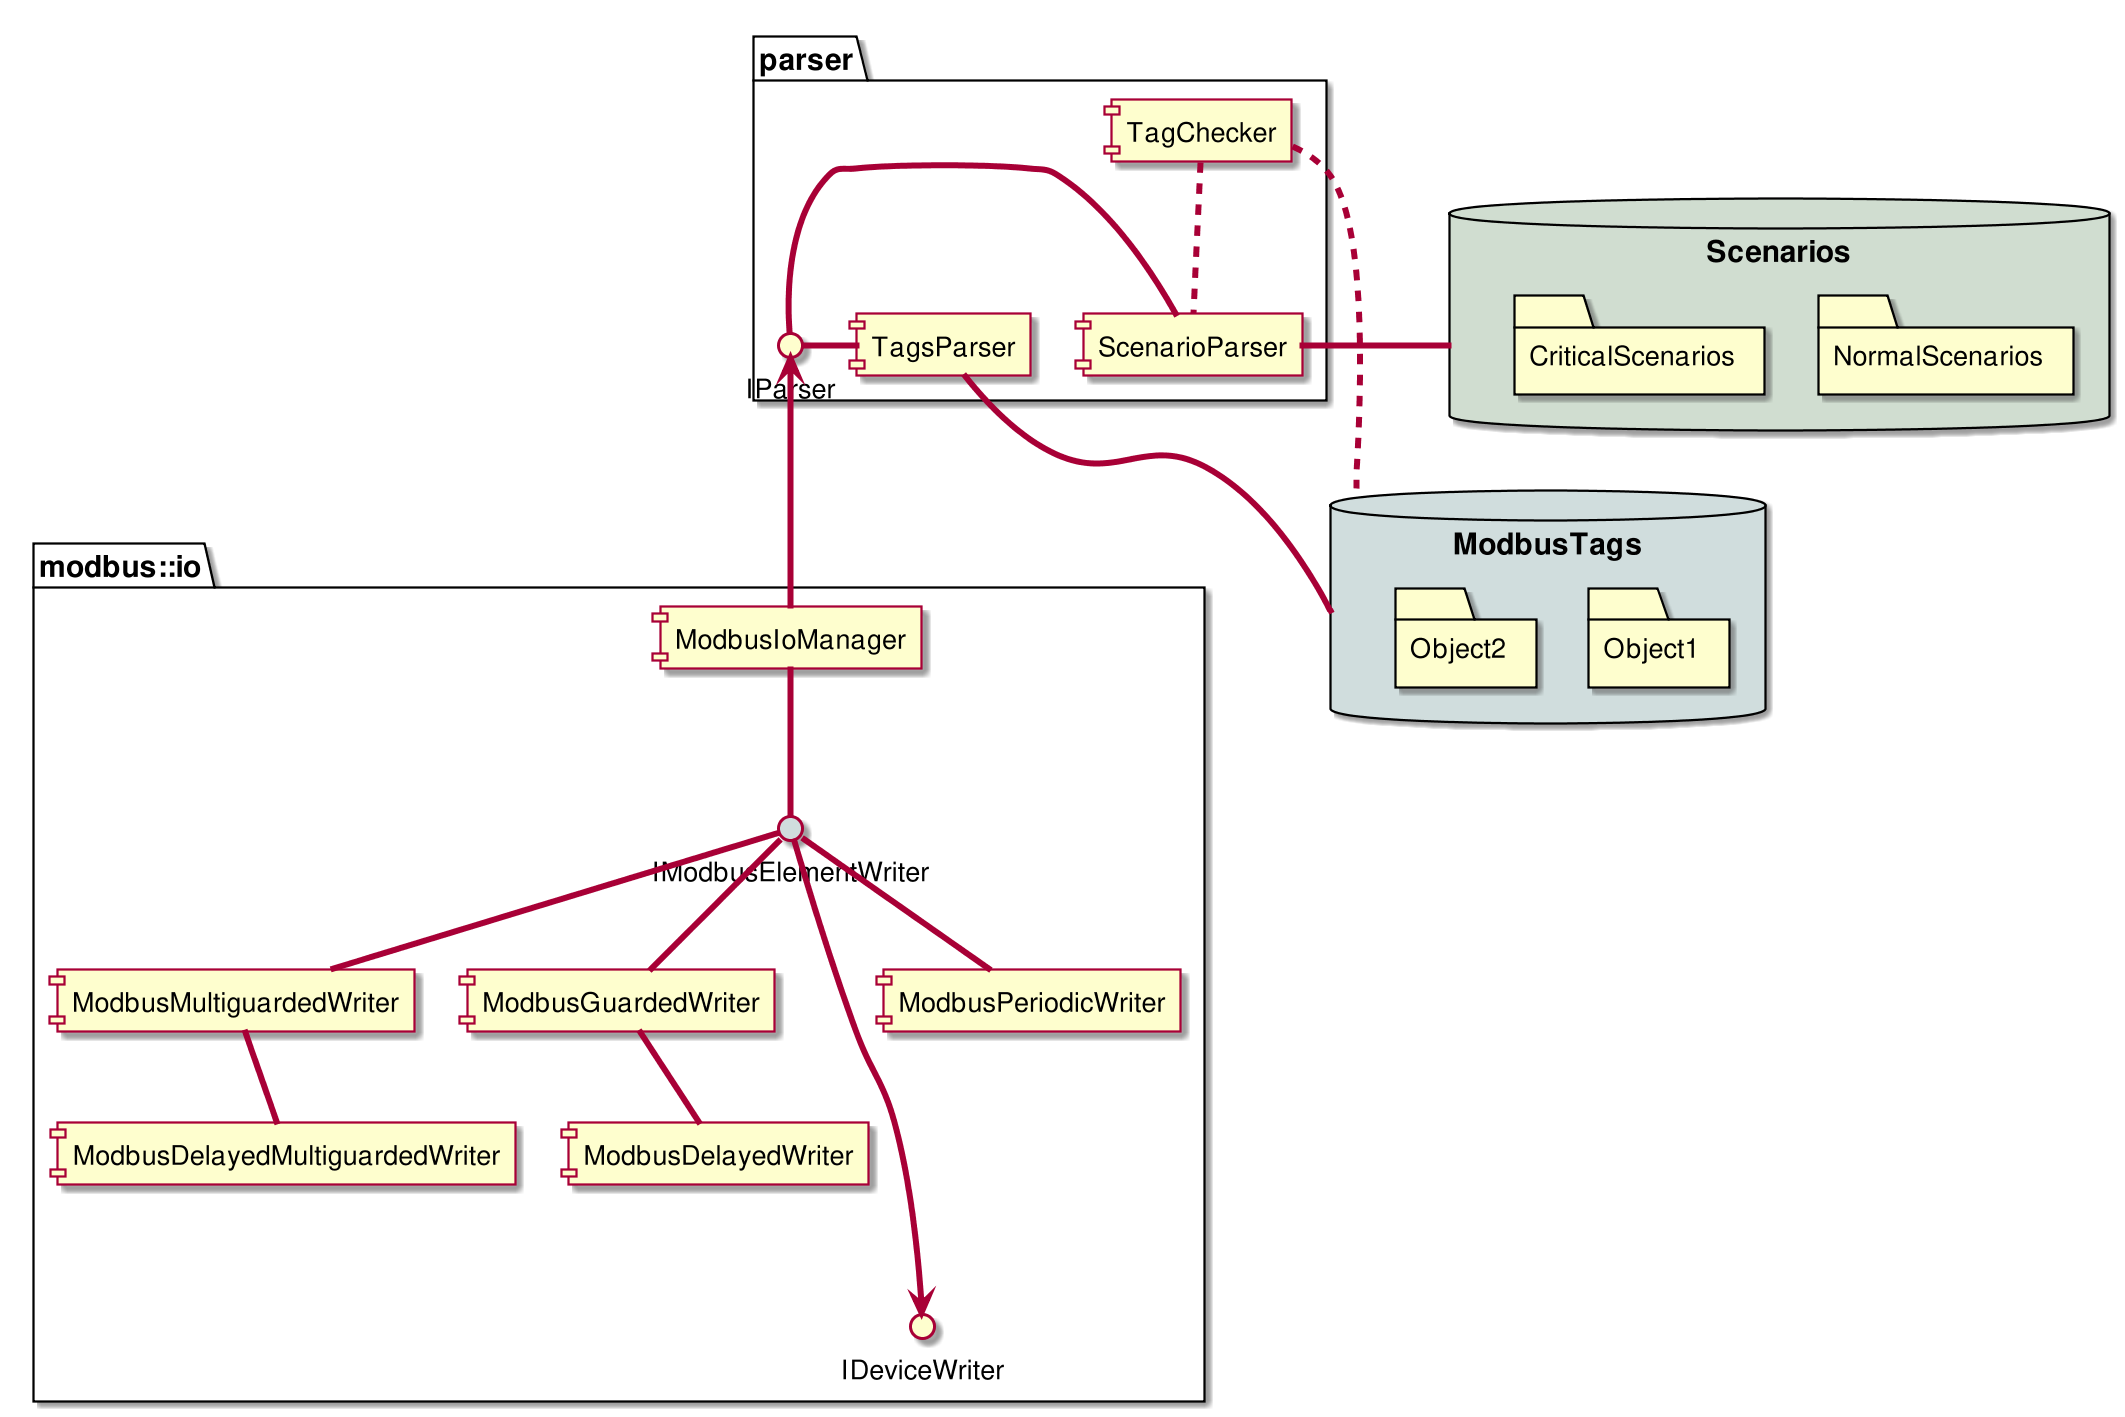
\includegraphics[width=.9\textwidth,keepaspectratio]{modbus_class_components}
        \caption{Композиция классов менеджера сценариев}\label{fig:modbus_class_components}
    \end{figure}
\end{center}


Последовательность действий по конфигурированию окружения программного обеспечения
показана на рисунке \ref{fig:top_level_sequence} \cite[стр. 239]{book:oop:oop_analize}.
\begin{center}
    \begin{figure}
        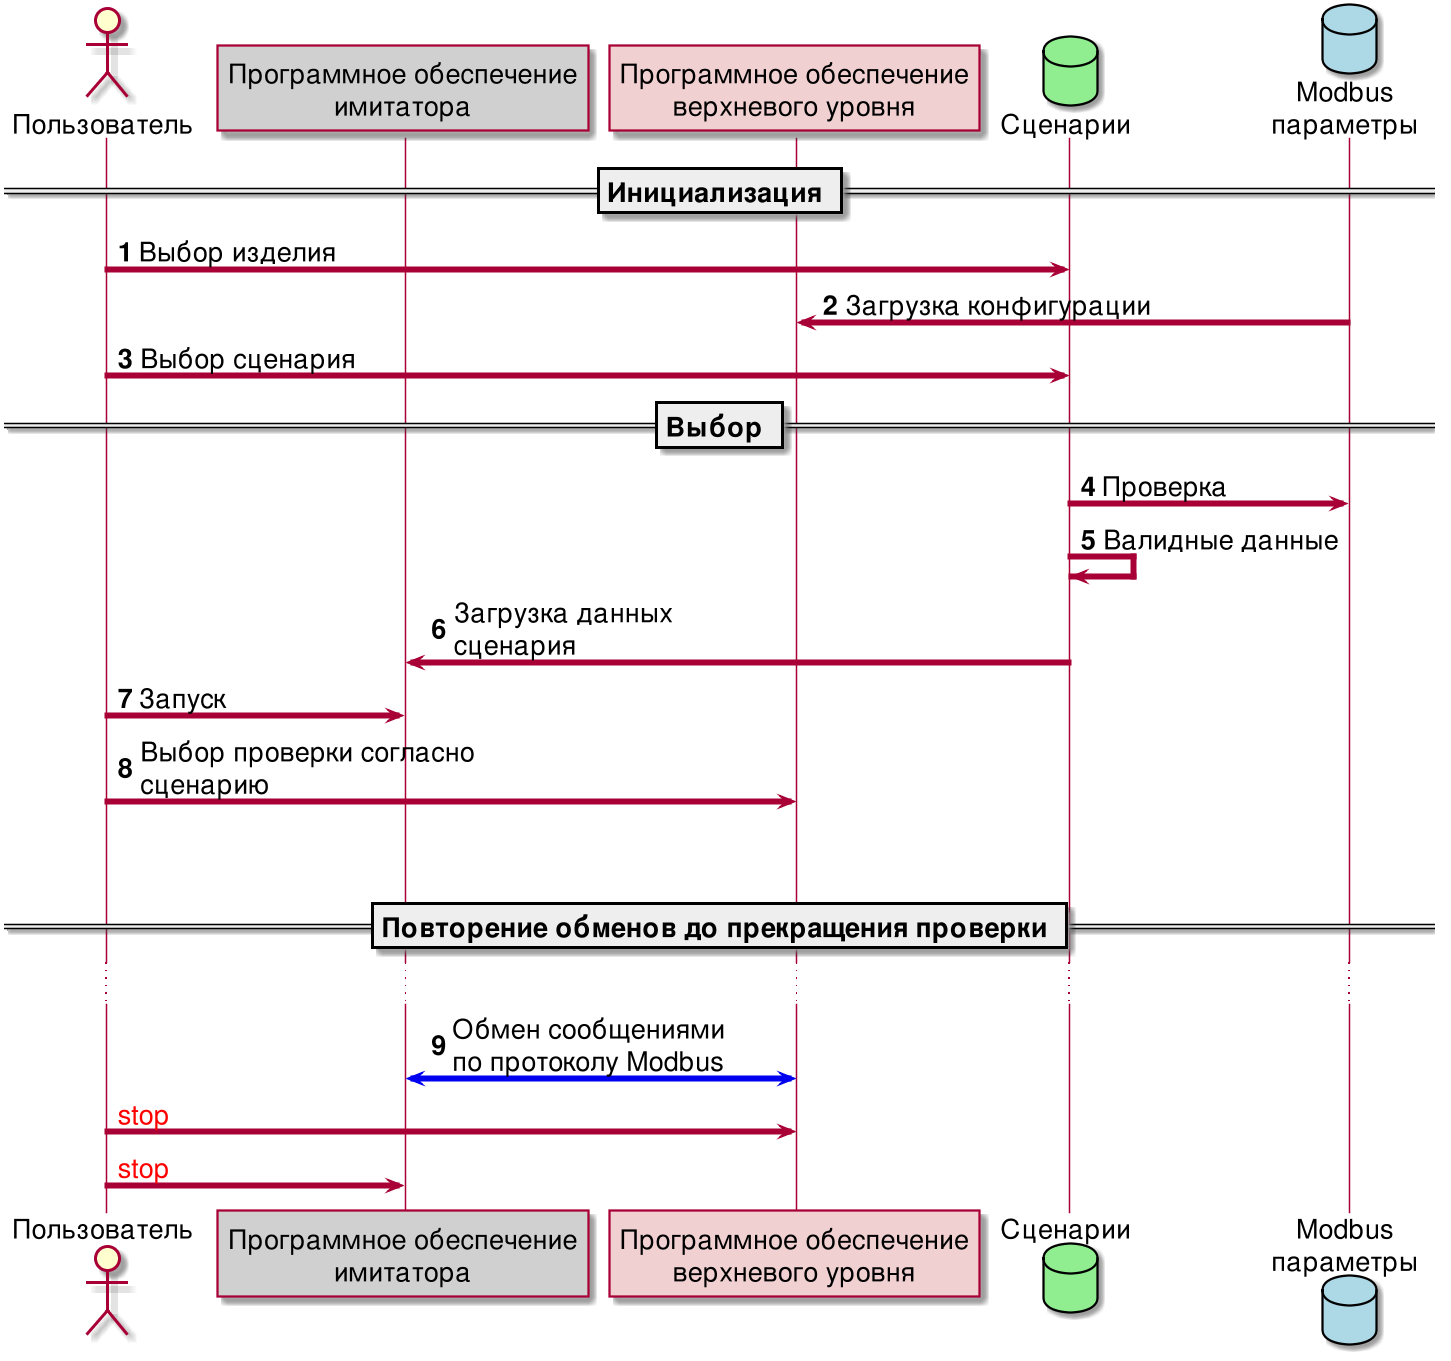
\includegraphics[width=.9\textwidth,keepaspectratio]{top_level.png}
        \caption{Последовательность действий при работе с имитатором}
        \label{fig:top_level_sequence}
    \end{figure}
\end{center}

\textbf{Инициализация и загрузка конфигурации.}
На этом этапе происходит настройка программного обеспечения
имитатора и программы, так называемого, верхнего уровня,
то есть программного обеспечения непосредственно системы контроля.
В случае корректной конфигурации происходит запуск
выбранной проверки оператором.

\textbf{Выполнение сценария проверки.}
После запуска две программы начинают обмениваться 
сообщениями по протоколу Modbus~TCP/IP, например внутри локальной сети.
Более подробно этот этап показан на рисунке \ref{fig:modbuselementwriterimpl}.

\textbf{Окончание проверки.}
Происходит возврат к исходным настройкам систем и отключение.
После этого процедура может быть воспроизведена вновь с теми же
или другими параметрами. 

\begin{center}
    \begin{figure}
        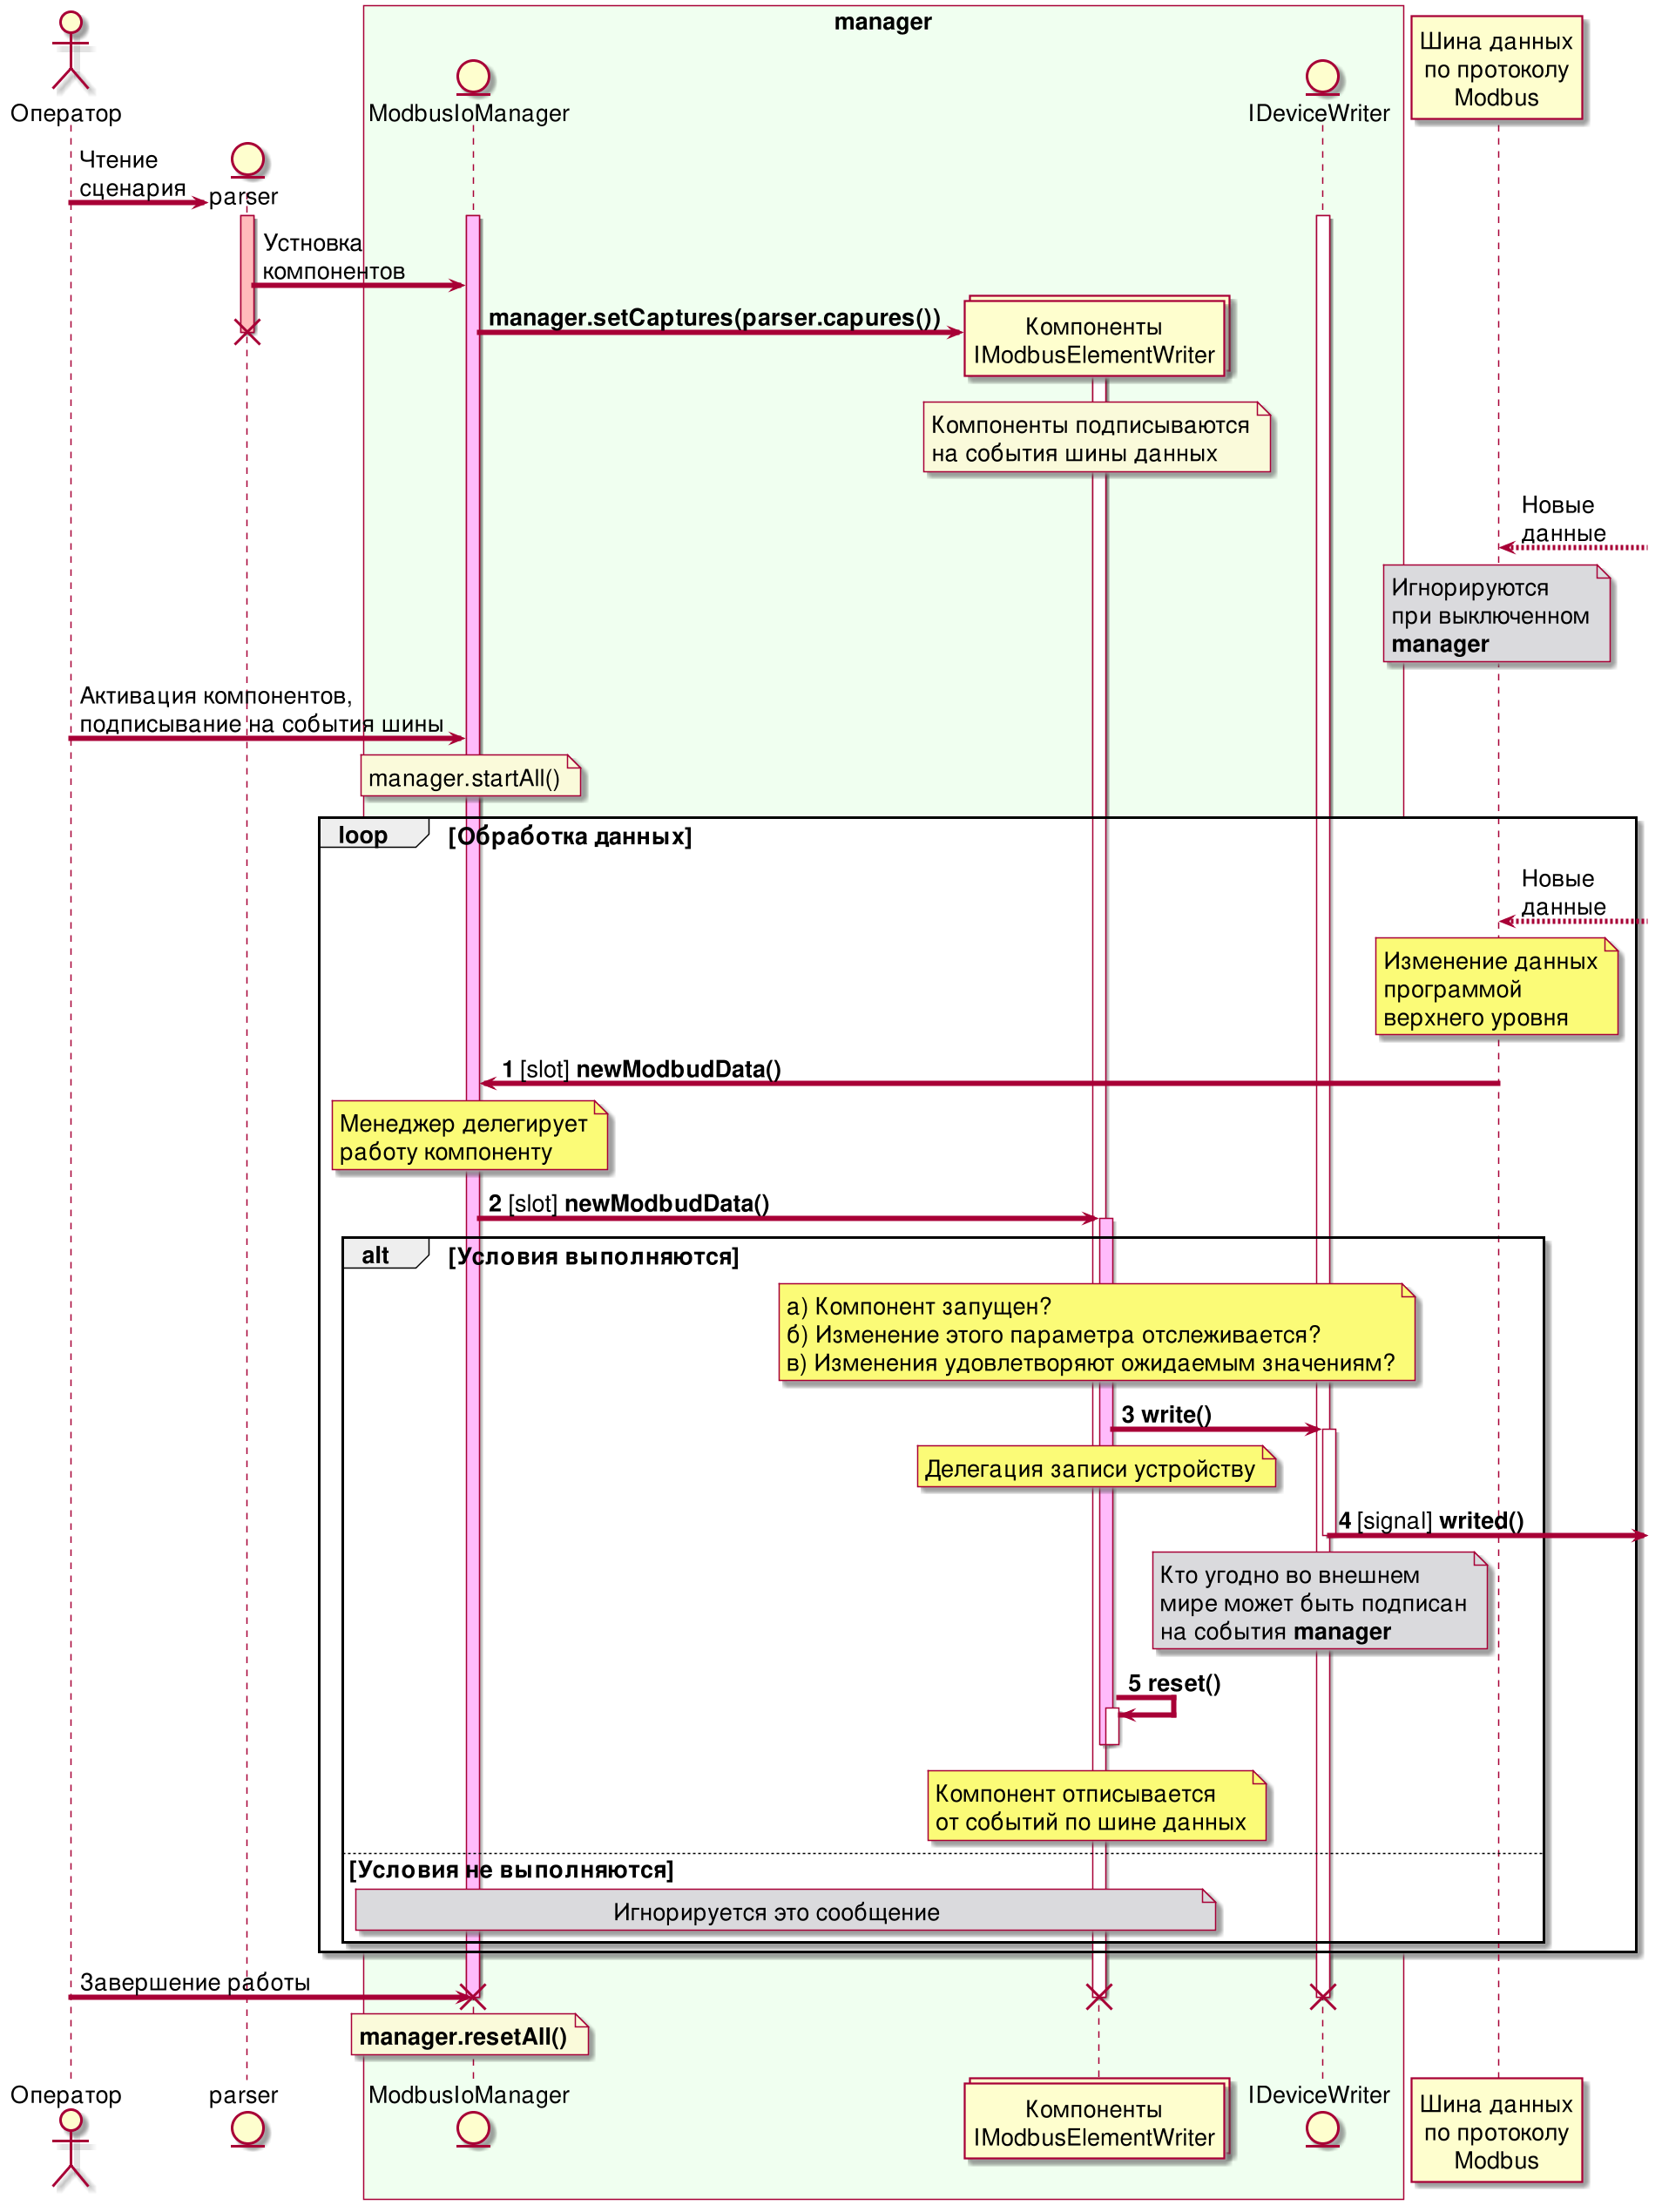
\includegraphics[height=.8\textheight,keepaspectratio]{modbuselementwriterimpl.png}
        \caption{Взаимодействие компонентов с шиной данных (см. также листинг \ref{lst:tmpl_method_writerimpl})}
        \label{fig:modbuselementwriterimpl}
    \end{figure}
\end{center}


\textbf{Обработка данных при выполнении сценария проверки.}
Как было сказано ранее, после запуска менеджера \texttt{modbusio::ModbusIoManager::startAll()}
менеджер готов к обработке данных.
До этого момента приходящие сообщения игнорируются им.

Таким образом, менеджер подписывается на изменения данных по шине Modbus,
через слот \texttt{newModbusData()}.
Работа с поступающими данными делегируется экземплярам, реализующих интерфейс
\texttt{IModbusElementWriter}, после чего происходит проверка поступающих данных
по следющим пунктам.
\begin{enumerate}
    \item Запущен ли компонент.
    \item Изменение это параметра отслеживается. Как было сказано ранее в разделе \ref{sec:ontology}
        два и более компонентов могут быть изоморфны относительно входного сигнала,
        таким образом, очевидно что этот сигнал перенаправляется всем компонентам,
        которыми владеет менеджер.
    \item Происходит проверка все ли предикаты в правилах перехода в значении истина. 
\end{enumerate}
При выполнении всех трех пунктов хотя бы для одного компонента,
происходит запись значения $P(x_1, \ldots, x_n) \to Q(x)$.
Компонент делегирует это экземпляру, реализующему интерфейс \texttt{IDeviceWriter},
через вызов виртуальной функции \texttt{IDeviceWriter::write()}.
В следствии этого компонент отписывается от событий по шине данных,
вызовом функции \texttt{IModbusElementWriter::reset()}.

Обработка данных при выполнении сценария проверки происходит до тех пор
пока менеджер не будет остановлен \texttt{ModbusIoManager::resetAll()}.


\section{Пример композиции для простейшего сценария}

Рассмотрим пример сценария на основе множества Modbus тегов из листинга \ref{lst:modbus_tags_example},
циклограмма которого представлена на рисунке \ref{fig:modbus_scenario_example_diagram},
сценарий приведен в листинге \ref{lst:modbus_scenario_example_diagram} в разделе приложения \ref{app:sec:modbus_scenario_example_diagram}.
Схема разметки приведена в листинге \ref{lst:modbus_tags_scenario_configs}.

\begin{landscape}
    \begin{center}
        \begin{figure}
            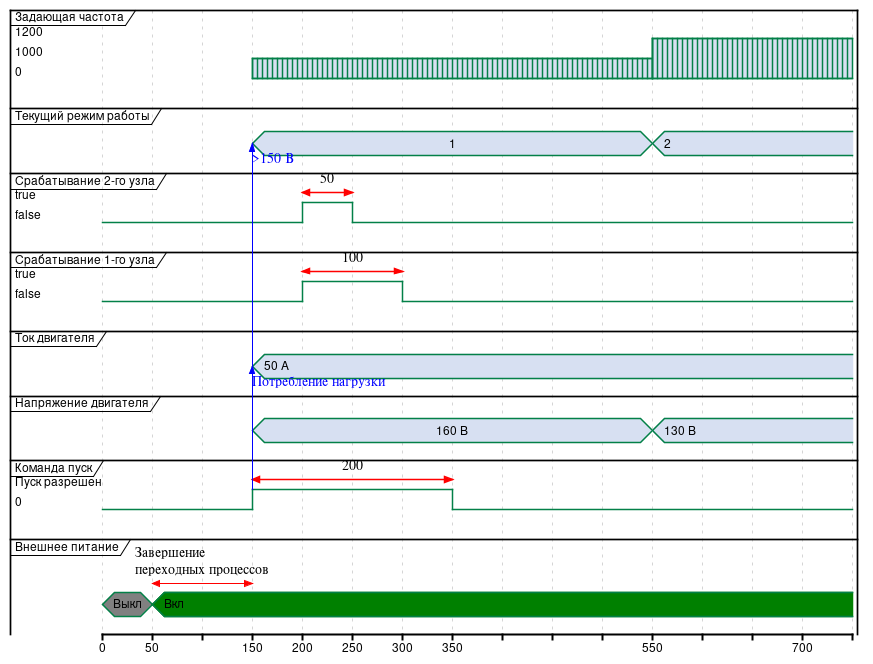
\includegraphics[height=.8\textheight,keepaspectratio]{modbus_scenario_example_diagram.png}
            \caption{Пример использования классов.}\label{fig:modbus_scenario_example_diagram}
        \end{figure}
    \end{center}
\end{landscape}
